
\vspace{-.5em}
\section{Method}
\vspace{-.5em}

\subsection{Overall}
\vspace{-.5em}

Given a raster image, our goal is to efficiently vectorize it into a VG representation that closely resembles the input while preserving the details. Existing methods, including DiffVG \cite{Li:2020:DVG} and its following work \cite{xu2022live, Chen_2024_CVPR}, incur substantial computational costs due to the pixel color accumulation computation. Specifically, DiffVG first constructs a bounding volume hierarchy (BVH) tree to determine the curves that intersect with each individual pixel, then solves equations to precisely determine whether a pixel lies within a region and to compute the inward or outward gradients at boundary points. 


To overcome this inefficiency, this work proposes a novel VG representation, Bézier Splatting, which is inspired by the high computational efficiency and expressive fitting capacity of Gaussian splatting \cite{zhang2024gaussianimage} for rasterization. Bézier Splatting \textit{samples 2D Gaussian points along Bézier curves and their interior regions}, then \textit{leverages
the Gaussian splatting method for efficient rasterization}, enjoying the following advantages:
\begin{itemize}\setlength{\itemsep}{3pt}
    \item This design significantly accelerates the forward and backward pass of Bézier curve rasterization, achieving an order-of-magnitude speedup without specialized optimization techniques;
    \item The 2D Gaussian representation inherently provides direct position gradients for object boundaries, eliminating the need for additional computations such as boundary sampling and gradient derivation via the Reynolds transport theorem in DiffVG \cite{Li:2020:DVG};
    \item It supports richer texture representation by allowing properties such as spatially varying opacity and width, facilitating complex effects such as linear-gradient color transitions within a single curve.
\end{itemize}
To further improve the fidelity and expressiveness of Bézier Splatting, we introduce a pruning and densification approach (Sec. \ref{sec:optimization}), which dynamically removes redundant Bézier curves while adaptively adding necessary curves in regions that have high reconstruction error. Fig. \ref{fig:framework} illustrates the algorithm flow of Bézier Splatting. More details are discussed in the following sections.

\begin{figure*}[t]
\centering
% \vspace{-.5em}
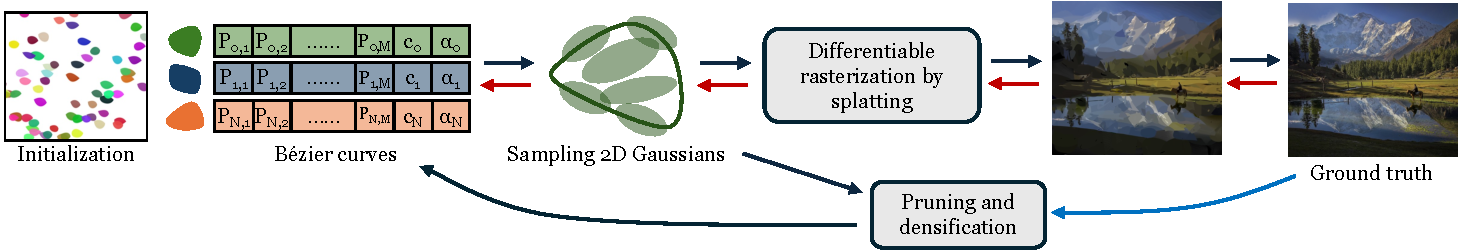
\includegraphics[width=1\linewidth]{figures/framework.pdf}
\caption{An illustration of the algorithm flow of Bézier Splatting. It begins by randomly initializing Bézier curves and uniformly sampling Gaussians points along them. These Gaussians are then rasterized into the image, enabling gradient-based computation to optimize parameters of both Bézier curves and Gaussians. Curves with negligible opacity or extremely small shapes are removed, while new curves are adaptively added into areas with high reconstruction error, ensuring curves are placed in areas requiring finer details. 
% rather than well reconstructed ones.
\textcolor{black}{$\rightarrow$} {forward}, 
\textcolor{red}{$\leftarrow$} backpropagation,
\textcolor{blue}{$\leftarrow$} error map.
}
\label{fig:framework}
\vspace{-.5em}
\end{figure*}

\vspace{-.5em}
\subsection{Primitives of Bézier Splatting}
\vspace{-.5em}

\noindent\textbf{Bézier curves.} We adopt Bézier curves as the parametric primitives of VGs. The representation includes \( N \) Bézier curves with a degree of \( M \), as:  
\begin{equation}
\mathcal{B}_i(t) = \sum_{j=0}^{M} B_j^M(t) P^{(i)}_{j}, \; t \in [0,1], \; i \in \{1, \dots, N\},
\label{eq:bezier}
\end{equation}
where $t$ is a normalized position on the curve, \( P^{(i)}_{j} \) represents the \( j \)-th control point of the \( i \)-th Bézier curve, and \( B_j^M(t) \) is the Bernstein polynomial of degree \( M \), given by:  
\begin{equation}
B_j^M(t) = \binom{M}{j} (1 - t)^{M-j} t^j.
\label{eq:bezier1}
\end{equation}
Each Bézier curve \( \mathcal{B}_i(t) \) is associated with an RGB color parameter \( c_i \in \mathbb{R}^3 \), and an opacity parameter \( o_i \in [0,1] \) that defines the transparency of the curve.


To formulate an open curve, we follow DiffVG \cite{Li:2020:DVG} to adopt three sequentially connected Bézier curves with two control points on each. An open curve requires an additional width parameter to define the stroke thickness.
For a closed curve, we adopt two connected Bézier curves, enabling a more efficient sampling in enclosed regions. For closed curves, color filling is applied. The connected Bézier curves in either an open or closed curve share the color parameters, but they have separate opacity parameters to better model the opacity changes along the curves or within closed areas for enriching the texture representation capacity. 

\noindent\textbf{2D Gaussians on curves.}  
Our Bézier Splatting novelly associates 2D Gaussians with each Bézier curve. The standard formulation of 2DGS \cite{Huang2DGS2024} parameterizes each 2D Gaussian by position, color, rotation, scale, opacity, and depth.
However, to ensure a compact and differentiable representation, these parameters of Gaussians in our Bézier Splatting are inherited from the corresponding control points. We discuss more details of the sampling of Gaussians, rasterization process, and backaward computation in the following sections.


\vspace{-.5em}
\subsection{Sampling Gaussians on Bézier Curves}
\vspace{-.5em}

This work introduces a fast differentiable VG rasterizer based on Gaussian splatting, allowing gradients from raster images to be backpropagated to the 2D Gaussians, then further backpropagated to the Bézier curves through a differentiable sampling strategy, resulting in a highly efficient optimization of the Bézier curves.  


Specifically, for each Bézier curve $\mathcal{B}_i(t)$, we uniformly sample $K$ points along it based on Eq. \ref{eq:bezier}. The sampled point set $\mathbf{b}_i$ is: 
\begin{equation}
\mathbf{b}_i = \big[ \mathcal{B}_i(t_0), \mathcal{B}_i(t_1), \dots, \mathcal{B}_i(t_{K-1}) \big],
\label{eq:sampling}
\end{equation}
where $t_k$ is uniformly sampled from \([0,1]\).

\noindent\textbf{Sampling 2D Gaussians on open curves.} We represent an open curve by using $3$ sequential Bézier curves $\mathcal{B}_i(t)$ with a degree of $4$ to form a single continuous stroke, by following the same setting as DiffVG \cite{Li:2020:DVG}. The stroke consists of 10 control points, as the end point of each Bézier curve serves as the start point of the next. To ensure that the final rendering result generates a continuous stroke with consistent width and color, we calculate the x-direction scale of a Gaussian point by the distance between neighboring points by following Eq. \ref{eq:sigma}, while the y-direction scale is a learnable parameter that represents the stroke width. 

For both closed and open curves, the depth $d$ of a Gaussian is assigned based on the area of curves, ensuring smaller curves are not occluded by larger ones. It prevents them from being ignored during optimization, as the gradient would not count Gaussians when the accumulated opacity exceeds 1.

\noindent\textbf{Sampling 2D Gaussians on closed curves.} Achieving accurate color filling is non-trivial for closed curves. A straightforward approach involves uniformly sampling a large number of points, identifying intersecting curves, solving equations to determine which curves cover them, and then computing scaling factors based on the sampled points. However, this process is computationally expensive, making it inefficient for curve rasterization and optimization.

% To address this limitation, we propose a new structure named \emph{paired Bézier curve structure} that facilitates an efficient closed area sampling between two Bézier curves of a closed curve. Specifically, the two Bézier curves \( \mathcal{B}_1(t) \) and \( \mathcal{B}_{R+1}(t) \) share the same start and end points, and $R$ intermediate Bézier curves are generated by interpolating the control points between the two Bézier curves $P^{(0)}_j$ and $P^{(R+1)}_j$as:
% \begin{equation}
% P^{(k)}_j = (1 - t_k) P^{(0)}_j + t_k P^{(R+1)}_j, \; k = 1, \dots, R,
% \end{equation}

To address this limitation, we propose a new structure named \emph{paired Bézier curve structure}, which supports two groups of Bézier curves with equal cardinality and arbitrary degrees, forming a closed region. This structure enables efficient and flexible sampling within the enclosed region between the two curve groups. Specifically, the two Bézier curves \( \mathcal{B}_1(t) \) and \( \mathcal{B}_{R+1}(t) \) share the same start and end points, forming the inside curves and boundaries of a closed region. A total of \( R \) intermediate Bézier curves are generated by linearly interpolating the corresponding control points \( P^{(0)}_j \) and \( P^{(R+1)}_j \) as:
\begin{equation}
P^{(k)}_j = (1 - t_k) P^{(0)}_j + t_k P^{(R+1)}_j, \quad k = 1, \dots, R,
\end{equation}
where \( t_k \in [0,1] \) are sampled from a normalized cumulative distribution function (CDF). The interpolated control points \( \{ P^{(k)}_j \} \) define intermediate curves that form a dense strip between the two boundaries. Note that this paired structure can naturally extend to cases where each curve is composed of multiple connected Bézier segments, provided that all segments have the same number of control points, similar to the representation used in DiffVG~\cite{Li:2020:DVG}.

This non-uniform sampling ensures that points near the boundary curves have small scales, mitigating the influence of interior Gaussians to the exterior of closed area. The interpolated Bézier curves are:
\begin{equation}
\mathcal{B}_k^{\text{interp}}(t) = \sum_{j=0}^{M} B_j^M(t) P^{(k)}_j, \quad k = 1, \dots, R.
\end{equation}
Then, 2D Gaussians are sampled on these interpolated curves, by following the same procedure as open curves (Eq. \ref{eq:sampling}), resulting in a structured and efficient point sampling within the enclosed region. Furthermore, to mitigate artifacts caused by non-convex curve shapes during interpolation, we incorporate the Xing loss from LIVE \cite{xu2022live}, which enforces convexity constraints on curve shapes, to improve the stability of the interpolation process.
The full set of sampled points on the $i$-th Bézier curve is:
\begin{equation}
\mathbf{X} = \big[ \mathbf{b}_0, \mathbf{b}_1, \dots, \mathbf{b}_{R+1} \big] \in \mathbb{R}^{{(R+2)} \times K \times 2}.
\end{equation}

% Let $\mathbf{X}_{r,k}$ represents the 2D position of the $k$-th sampled point on the $r$-th interpolated curve, the x-direction scale $\sigma_x(r,k)$ of a 2D Gaussian is calculated by the pairwise distance between consecutive points along the curve, and y-direction scale $\sigma_y(r,k)$ is calculated by the pairwise distance between corresponding points on adjacent curves:
% \begin{equation} \label{eq:sigma}
% \begin{aligned}
% \sigma_x(r,k) &= \| \mathbf{X}_{r,k+1} - \mathbf{X}_{r,k} \|_2 / \rho, \\
% \sigma_y(r,k) &= \| \mathbf{X}_{r+1,k} - \mathbf{X}_{r,k} \|_2 / \rho.
% \end{aligned}
% \end{equation}
% $\rho$ is a constant that determines the density of 2D Gaussian points.
% The rotation $\theta$ of each Gaussian point is calculated by its left and right neighbors, as \begin{equation} \theta_{r,k} = \operatorname{atan2}\left( y_{r,k+1} - y_{r,k-1}, x_{r,k+1} - x_{r,k-1} \right) \label{eq:rotation} \end{equation}
% For points on boundaries, the rotation is set to align with the nearest neighbor.

Let $\mathbf{X}_{r,k}$ denote the 2D position of the $k$-th sampled point on the $r$-th interpolated curve.
To construct anisotropic 2D Gaussian primitives aligned with the local geometry, we define the spatial scales as follows.
The \emph{x-direction} of each 2D Gaussian is defined to align with the local tangent direction of the curve (i.e., along the curve),
while the \emph{y-direction} is perpendicular to it (i.e., across adjacent curves).

The scale $\sigma_x(r,k)$ is computed from the Euclidean distance between consecutive points along the curve, and $\sigma_y(r,k)$ is computed from the distance between corresponding points on adjacent curves:
\begin{equation} \label{eq:sigma}
\begin{aligned}
\sigma_x(r,k) &= | \mathbf{X}_{r,k+1} - \mathbf{X}_{r,k} |_2 / \rho, \\
\sigma_y(r,k) &= | \mathbf{X}_{r+1,k} - \mathbf{X}_{r,k} |_2 / \rho.
\end{aligned}
\end{equation}
Here, $\rho$ is a global constant that controls the overall density and overlap of the Gaussians.
The rotation $\theta_{r,k}$ of each Gaussian is defined by the angle of the local tangent vector, estimated from neighboring points as
\begin{equation} \label{eq:rotation}
\theta_{r,k} = \operatorname{atan2}\left( y_{r,k+1} - y_{r,k-1}, x_{r,k+1} - x_{r,k-1} \right).
\end{equation}
For boundary points, the rotation is set to align with the nearest available neighbor.




\vspace{-.5em}
\subsection{Splatting-based Differentiable Rasterization}
\vspace{-.5em}

\label{sec:rasterizer}
Once all Gaussians on Bézier curves are sampled, the rasterization process follows the Gaussian splatting pipeline \cite{kerbl3Dgaussians}, which is very fast in both forward and backward computation. Different from GaussianImage \cite{zhang2024gaussianimage}, we use $\alpha$-blending for pixel rendering instead of the accumulation-based blending. 
Accumulation-based blending calculates the pixel value based on all overlapping Gaussians, such that it conflicts with the rendering principles of VGs, where occlusion plays a crucial role in defining vector structures.
$\alpha$-blending ensures proper occlusion handling, as it allows foreground elements to contribute more to the final pixel value. 
The rendering of a pixel is:
\begin{equation}
    C_n = \sum_{i \in M}\mathbf{c}_i\alpha_i \prod_{j=1}^{i-1}(1 - \alpha_j).
\end{equation} 
$C_n$ is the $n$-th pixel color, $\mathbf{c}_i$ is the color of corresponding Gaussians, $\alpha_i$ is computed by the projected 2D covariance $\Sigma_i$:
\begin{equation}
\alpha_i = o_i \exp^{-\sigma_i}, \quad 
\sigma_i = \frac{1}{2} \boldsymbol{d}_n^T \boldsymbol{\Sigma}^{-1}_{i} \boldsymbol{d}_n.
\label{eq:rasterization2}
\end{equation}
where $d_n$ is the distance between the pixel and Gaussian center, and $\Sigma_i$ can be modeled by $\theta_i$, $\sigma_x^i$ and $\sigma_y^i$ as:
\begin{equation}
\boldsymbol{\Sigma}_i = (\boldsymbol{R}_i \boldsymbol{S}_i)(\boldsymbol{R}_i \boldsymbol{S}_i)^T.
\label{eq:RSSR}
\end{equation}
\begin{equation}
\boldsymbol{R}_i =
\begin{bmatrix}
\cos(\theta_i) & -\sin(\theta_i) \\
\sin(\theta_i) & \cos(\theta_i)
\end{bmatrix},
\quad
\boldsymbol{S}_i =
\begin{bmatrix}
\sigma_{x}^i & 0 \\
0 & \sigma_{y}^i
\end{bmatrix}.
\label{eq:rot_scale}
\end{equation}

\noindent\textbf{Discussion on method efficiency.}
The rasterization process of Bézier Splatting is very efficient, since we directly sample 2D Gaussians from Bézier curves in a differentiable manner, then splat them to the 2D plane. The rasterization pipeline remains end-to-end differentiable while being highly optimized for parallel computation and large-scale matrix operations.
As a result, Bézier Splatting is a highly efficient and fully differentiable VG representation, which ensures both fast rendering and gradient-based optimization. It not only preserves the flexibility of VGs but also allows seamless integration into deep learning frameworks, making it well-suited for tasks requiring high-quality and editable vector representations.


\vspace{-.5em}
\subsection{Optimization}
\vspace{-.5em}
\label{sec:optimization}

\noindent\textbf{Training objective.}
Given a raster image $\mathcal{I} \in \mathbb{R}^{H \times W \times 3}$, the goal of image vectorization is to vectorize the image into Bézier curves while ensuring a high-fidelity reconstruction. We first randomly generate a set of Bézier curves to lay on the canvas, then employ the differentiable rasterizer discussed in Sec. \ref{sec:rasterizer} to render a raster image $\hat{\mathcal{I}} \in \mathbb{R}^{H \times W \times 3}$. The Bézier curves can then be optimized through any gradient-based loss functions. 
In this work, we formulate the optimization objective as minimizing the loss between  $\mathcal{I}$ and $\hat{\mathcal{I}}$ while enforcing the curves to be convex. Therefore, we only adopt an $L_2$ loss and a Xing loss $L_{\text{Xing}}$  \cite{xu2022live}, as:
\begin{equation}
L = \lambda_1 \|\hat{\mathcal{I}} - \mathcal{I} \|_2^2 +  \lambda_2 L_{\text{Xing}}
\end{equation}
where $\lambda_1$ and $\lambda_2$ are hyperparameters that trade off the two loss functions.



\noindent\textbf{Adaptive curve pruning and densification.}
The gradients of 2D Gaussians are influenced by local pixels only. Therefore, it is hard for 2D Gaussians to dynamically reallocate to regions requiring finer-grained details. The Gaussians would be trapped in local minima, leading to redundant Gaussians that are optimized as either low opacity or excessively large size, resulting in artifacts in rendering results. 

In standard 3D Gaussian Splatting pipeline \cite{kerbl3Dgaussians}, Gaussians with low opacity or excessive size are pruned, whereas those with high gradient responses are split into two. However, this strategy is not directly applicable to Bézier curves. Note that in volumetric representations, large Gaussians are usually unnecessary for modeling any particular structure. In contrast, VG representations often encompass large uniform regions such as backgrounds or areas with homogeneous colors (\textit{e.g.,} walls). Consequently, the size-based pruning strategy would remove critical structures in VG representations. Similarly, splitting a Bézier curve into two can introduce significant randomness, as high-gradient regions do not always indicate poor reconstruction in VGs. Since VGs assume a uniform color within each enclosed region, complex textures naturally produce high gradients. This does not imply the region should be split, as it may disrupt the semantic consistency of the VG representation.



To address this issue, this work introduces a new pruning and densification strategy to dynamically adjust the density of Bézier curves throughout the optimization process. For pruning redundant Bézier curves, we apply three criteria to ensure a stable and precise optimization process. First, we remove curves with opacity below a dynamic threshold that gradually decreases as optimization progresses, ensuring that weakly contributing curves are eliminated while preserving essential structures. Second, we remove curves with an area below a predefined threshold, as they contribute minimally to the final representation. To remove visually insignificant or noisy Bézier curves, we apply an opacity-based filtering strategy: for per-segment opacities, we discard curves whose middle segment is significantly fainter than both ends—often indicating that a single curve improperly spans a region better represented by multiple curves; otherwise, we discard curves with overall opacity below a threshold (e.g., 0.2) to eliminate globally low-visibility curves. Third, we remove curves that exhibit high color similarity with surrounding curves and have significant overlap, as they provide little additional information and can be pruned without affecting the final representation. By removing such curves, we allow the optimization to introduce more appropriate replacements, leading to a more accurate and visually coherent vectorized representation. For curve densification, we adopt an error-driven curve allocation strategy inspired by LIVE \cite{xu2022live}. Specifically, we compute connected error regions, rank them by area, and add new Bézier curves into the highest-error regions. This adaptive redistribution mechanism ensures that curves are allocated to where they would contribute the most to the reconstruction fidelity. The pruning and densification strategy enables a ``global receptive field'' for redistributing curve density, effectively preserving visual details for high-fidelity rendering while maintaining a compact vector representation.